\documentclass[12pt]{article}
\usepackage[T1]{fontenc}
%\usepackage[latin9]{inputenc}
\usepackage[utf8]{inputenc}
\usepackage[english]{babel}
\usepackage{amsmath}
\usepackage{amsfonts}
\usepackage{amssymb}
\usepackage{setspace}
\usepackage{rotating}
\usepackage{graphics}
\usepackage{eurosym}
\usepackage[round]{natbib}
%\usepackage{graphicx}
%\usepackage{float} 				%allows you to float images
\usepackage{latexsym}
\usepackage{bbding}
%\usepackage {moresize}
\usepackage{listings}
\usepackage{bbding}
\usepackage{blindtext}
\usepackage{hhline}
\usepackage{tikz}
\usetikzlibrary{trees}
%\usetikzlibrary{shapes,backgrounds}
%\usepackage{pgfplots}
%\usetikzlibrary{arrows}
\usepackage{enumitem}
\doublespacing
%\usepackage{geometry}
\usepackage{amsthm}
\usepackage{color}
%\usepackage{array,multirow}
%\usepackage{subcaption}
%\usepackage{pst-plot}
%	\psset{xunit=15mm}
%\geometry{verbose,tmargin=1in,bmargin=1in,lmargin=.5in,rmargin=.5in}
\setlength{\parskip}{\bigskipamount}
\setlength{\parindent}{0pt}
\usepackage{multicol}

\newenvironment{problem}[3][Problem]{\begin{trivlist}
\item[\hskip \labelsep {\bfseries #1}\hskip \labelsep {\bfseries #2.}]}{\end{trivlist}}

\newcommand{\barr}{\bar{r}}
\newcommand{\ddx}{\frac{d}{dx}}
\newcommand{\infsum}{\sum_{n=1}^{\infty }}

\title{Problem Set 9 \thanks{Problems:2,4,6,8,18}}
\author{Ian McGroarty \\
	Course Number: 625.641}
\date{July 30, 2019}

\begin{document}

\maketitle
\newpage
%%%%%%%%%%%%%%%%%%%%%%%%%%%%%%%%%%%%%%%%%%%%%%%%%%%%%%%%
%%%%%%%%%%%%%%%%%%%%%%%%%%%%%%%%%%%%%%%%%%%%%%%%%%%%%%%%
%%%%%%%%%%%%%%%%%%%%%%%%%%%%%%%%%%%%%%%%%%%%%%%%%%%%%%%%
\begin{problem}{2 (Proportional Carrying Charges)}. Suppose that a forward contract on an asset is written at time zero and there are M periods Carrying charge is $qS(k)$. 
\begin{center}
\begin{tabular}{c|c|c}
Period & Quantity & Carrying Cost \\ 
\hline
0 & $x_0 $ & $-S(0)$ \\ 
1  & $x_0 - qx_0 = x_0(1-q)$ & $-(S(0) + qS(0)= S(1-q)$ \\ 
2 & $x_0(1-q)^2 $ & $S(1-q)^2$ \\ 
$\vdots $ & $\vdots $ & $\vdots $ \\
 M & $x_0(1-q)^M $ & $S(0)$ - Repay 
\end{tabular}
\end{center}
\begin{align*}
Profit \; = \pi &= F\cdot Q - \frac{S }{d(0,M)}  && \text{Profit function} \\
F\cdot Q &= \frac{S }{d(0,M)} && \text{Set profit to zero} \\
F \cdot x_0(1-q)^M & = \frac{S}{d(0,M)} && \text{Substitute quantity at period M} \\
F &= \frac{S}{(1-q)^M \cdot d(0,M)} && \text{Set $x_0=1$ and solve} 
\end{align*}
  \end{problem}
%%%%%%%%%%%%%%%%%%%%%%%%%%%%%%%%%%%%%%%%%%%%%%%%%%%%%%%%
\newpage
\begin{problem}{4 (Continuous time Carrying Charge)}. Suppose continuous compounding framework is used with a fixed interest rate r. \\
So the interest rate will be the discount factor for continuous time (page 75) $d(0,M) = e^{-rM}$. We see that the relation between discrete time $(1+r)^M$ and continuous time $e^{rM}$ that quantity will be $e^{qm}$ Plugging these values into the result from problem 2 we get: $$ F= \frac{S}{e^{qM} \cdot e^{-rM}} = \frac{S}{e^{(q-r)M}} = Se^{(r-q)M} $$
\end{problem}

%%%%%%%%%%%%%%%%%%%%%%%%%%%%%%%%%%%%%%%%%%%%%%%%%%%%%%%%
\newpage
\begin{problem}{ 6 (Foreign Currency Alternative} The US electronics company received and order to sell equipment to a German customer in 90 days. Price specified as 500,000 D-Mark (wow this book is old) . To understand how to hedge the risk we must first understand the risk itself. Since the US firm will want to convert the payment into dollars, the true price that the US is receiving is 500,000 E where is is the exchange rate. If the value of the D-Mark goes down relative to the dollar, then the US will loose value on the transaction. If the value of the D-Mark goes up relative to the dollar then the US will make money on the transaction. Thus, the US is the 'natural long' in this scenario (see the graph below), with the asset D-Mark. By shorting the D-Mark the US hedges against risk.  If the D-Mark depreciates relative to the dollar, the short position will cover the losses from the transaction. Conversely, if the D-Mark appreciates relative to the dollar, the short position will lose money and thereby offset the gains of the transaction. 

As the problem states, there is another way to offset the exchange rate risk. By borrowing $500,000/(1+r_G)$ D-Mark and converting the money to USD and then into treasury bills. The firm effectively removes their dependency on the D-Mark since they paid themselves. If the D-Mark depreciates then the value of the loan also depreciates and vice versa. Note that they don't need to borrow the full 500,000 D-Mark since this reflects the present value of a bond with a face value of 500,000. \\
\begin{centering}
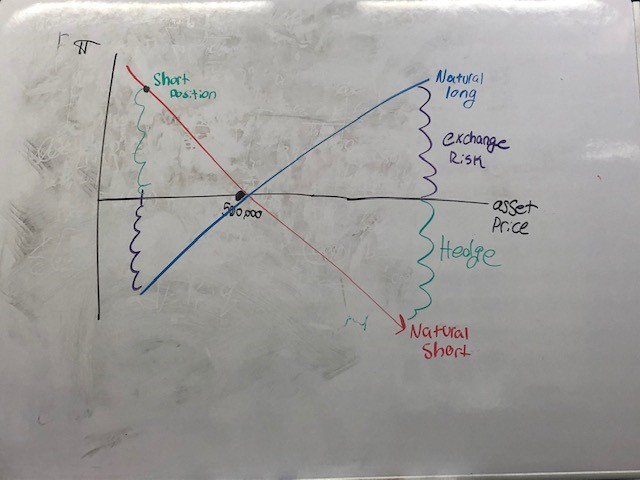
\includegraphics[width=\textwidth ]{mod9p6.jpg}
\end{centering}
\end{problem}

%%%%%%%%%%%%%%%%%%%%%%%%%%%%%%%%%%%%%%%%%%%%%%%%%%%%%%%%
\newpage
\begin{problem}{8 (Simple Formula)}.  Derive the formula (10.6) b converting a cash flow of a bond to that of the fixed portion of the swap. \\
\textbf{Solution} Note the the discount rate $d(0,M)=\frac{1}{(1+\lambda / m)^n}$. 
\begin{align*}
P &= \frac{F}{(1+\lambda / m)^n} + \Sigma \frac{C/m}{(1+\lambda / m)^n}  && \text{ (3.1) page 53} \\ 
P &= F(d(0,M)) + \Sigma (C/m)(d(0,M)) && \text{substitute} \\ 
P - F(d(0,M)) &= \Sigma (C/m)(d(0,M)) \\ 
P - F(d(0,M)) &= C \cdot \Sigma (d(0,M)) && \text{Since C is constant} \\ 
\frac{1}{C} (P - F(d(0,M)) &= \Sigma (d(0,M)) \\
\frac{X}{C} (P - F(d(0,M))&= \Sigma(d(0,M)) X &&\text{Multiply by x?} 
\end{align*}
Then we have $P=B(M,C)$ and $F=100$ as stated on page 275. 
\end{problem}

%%%%%%%%%%%%%%%%%%%%%%%%%%%%%%%%%%%%%%%%%%%%%%%%%%%%%%%%
\newpage
\begin{problem}{18 (Symmetric Probability)} Suppose the wealth that is to be received at a time T in the future has the following form. Where X is a random variable with $E(x)=0$: \\
\textbf{(a) Show that the optimal choice is} $h=0$. 
\begin{align*}
W &= a + hx + cx^2 \\
\ddx W &= \ddx a + hx + cx^2 && \text{take the derivative w respect to x} \\
0 &= h + 2cx && \text{Set to 0} \\
h &= 2cx
\end{align*}
It is clear that as $x \rightarrow 0 \implies h \rightarrow 0.$\\ 
\textbf{(b) Apply this result to the corn farm problem } 
\begin{align*}
R &= 10C - \frac{C^2}{1000} + \frac{\bar{C}-C}{1000}h && \text{page 29} \\
\ddx R &= \ddx 10C - \frac{C^2}{1000} + \frac{\bar{C}-C}{1000}h && \text{take the derivative w respect to C} \\
0&= 10 - \frac{2C}{1000} + \frac{h}{1000} && \text{Set to 0} \\
10000-2C &= h \\
10000 - 2(3000) &= h = 4000 && \bar{C} = 3000
\end{align*}

\end{problem}
\end{document}




% Set the overall layout of the tree




\tikzstyle{level 1}=[level distance=3.5cm, sibling distance=3.5cm]
\tikzstyle{level 2}=[level distance=3.5cm, sibling distance=2cm]

% Define styles for bags and leafs
\tikzstyle{bag} = [text width=4em, text centered]
\tikzstyle{end} = [circle, minimum width=3pt,fill, inner sep=0pt]

\begin{tikzpicture}[grow=right, sloped]
\node[bag] {Bag 1 $4W, 3B$}
    child {
        node[bag] {Bag 2 $4W, 5B$}        
            child {
                node[end, label=right:
                    {$P(W_1\cap W_2)=\frac{4}{7}\cdot\frac{4}{9}$}] {}
                edge from parent
                node[above] {$W$}
                node[below]  {$\frac{4}{9}$}
            }
            child {
                node[end, label=right:
                    {$P(W_1\cap B_2)=\frac{4}{7}\cdot\frac{5}{9}$}] {}
                edge from parent
                node[above] {$B$}
                node[below]  {$\frac{5}{9}$}
            }
            edge from parent 
            node[above] {$W$}
            node[below]  {$\frac{4}{7}$}
    }
    child {
        node[bag] {Bag 2 $3W, 6B$}        
        child {
                node[end, label=right:
                    {$P(B_1\cap W_2)=\frac{3}{7}\cdot\frac{3}{9}$}] {}
                edge from parent
                node[above] {$B$}
                node[below]  {$\frac{3}{9}$}
            }
            child {
                node[end, label=right:
                    {$P(B_1\cap B_2)=\frac{3}{7}\cdot\frac{6}{9}$}] {}
                edge from parent
                node[above] {$W$}
                node[below]  {$\frac{6}{9}$}
            }
        edge from parent         
            node[above] {$B$}
            node[below]  {$\frac{3}{7}$}
    };
\end{tikzpicture}


\section{Definitions}
\underline{Def: Forward Rate Formulas} (pg 79). The implied forward rate between times $t_1$ and $t_2$ is the rate of interset between those times that is consistent with a given spot rate curve. For Yearly compounding, the forward rate is:  
\begin{align*}
f_{i,j} =& [\frac{(1+s_j)^j}{(1+s_i)^i}]^{1/(j-i)}-1 \\
 e^{s(t_2)t_2} =& e^{s(t_1)t_1}e^{f_{t_1,t_2}(t_2-t_1)}
\end{align*}

\underline{Discount Factor Relation} The discount facot between periods i and j is defined as $$ d_{i,j}=[\frac{1}{1+f_{i,j}}]^{j-i}$$ These factors satisfy the compounding rule: $d_{i,k}=d_{i,j}d_{j,k}$\\

\underline{Def. Derivative (Ross pg 223)} Let F be a real valued function defined on an open interval contained a point a. We say f is differentiable at a, or f has derivative at a if the limit $$ f'(a) = \lim_{x \to a} \frac{f(x)-f(a)}{x-a} $$




https://www.investopedia.com/university/advancedbond/bond-pricing.asp
https://quant.stackexchange.com/questions/22288/duration-of-perpetual-bond
http://people.stern.nyu.edu/gyang/foundations/sample-final-solutions.html
http://pages.stern.nyu.edu/~jcarpen0/courses/b403333/07convexh.pdf
https://web.stanford.edu/class/msande247s/2009/summer%2009%20week%205/Bond%20Formula%20Sheet.pdf


\underline{Def: Forward Rate Formulas} (pg 79). The implied forward rate between times $t_1$ and $t_2$ is the rate of interset between those times that is consistent with a given spot rate curve. For Yearly compounding, the forward rate is:  
\begin{align*}
f_{i,j} =& [\frac{(1+s_j)^j}{(1+s_i)^i}]^{1/(j-i)}-1 \\
 e^{s(t_2)t_2} =& e^{s(t_1)t_1}e^{f_{t_1,t_2}(t_2-t_1)}
\end{align*}

\underline{Discount Factor Relation} The discount facot between periods i and j is defined as $$ d_{i,j}=[\frac{1}{1+f_{i,j}}]^{j-i}$$ These factors satisfy the compounding rule: $d_{i,k}=d_{i,j}d_{j,k}$\\

\underline{Def. Derivative (Ross pg 223)} Let F be a real valued function defined on an open interval contained a point a. We say f is differentiable at a, or f has derivative at a if the limit $$ f'(a) = \lim_{x \to a} \frac{f(x)-f(a)}{x-a} $$



\begin{align*}
\text{Maximize  } & 4x_1 +5x_2 +3x_3 +4.3x_4 + x_5 + 1.5x_6 + 2.5x_7 + 0.3x_8 + x_9 + 2x_{10} \\
\text{Subject to } & 2x_1 + 3x_2 + 1.5x_3 + 2.2x_4 +0.5x_5 +15x_6 + 2.5x_7 +0.1x_8 + 0.6x_9 + x_{10} \leq 5 \\ 
& x_1 + x_2 + x_3 + x_4 \leq 1 \\
& x_5 + x_6 + x_7 \leq 1 \\
& x_8 + x_9 + x_{10} \leq 1 \\
\end{align*}